% !TeX root = document.tex
% !TeX encoding = UTF-8 Unicode

\section{False Data Injection}%
\label{sec:fdi}

\subsection{Introduction}%
\label{subsec:fo-introduction}

\begin{slide}{}
  \usebeamercolor{frametitle}
  \vspace*{\fill}
  \begin{center}
    \textcolor{fg}{\Large{False Data Injection}}
  \end{center}
  \vspace*{\fill}
\end{slide}

\begin{slide}{False Data Injection}
  \begin{columns}[c]
    \begin{column}{0.48\textwidth}
      \begin{itemize}
        \item \textbf{False Data Injection}: the attacker changes the sensor
              reading sent over the network.
        \item Current detection schemes are mainly based on Kalman filters
              associated with residual generators, or IT-based techniques.
      \end{itemize}
    \end{column}%
    \hfill%
    \begin{column}{0.48\textwidth}
      \begin{align}
        \tilde{y}_{j} & = y_{i},            \\
        \tilde{y}_{j} & = y_{j}+\delta,     \\
        \tilde{y}_{j} & = y_{j}\cdot\alpha,
      \end{align}
    \end{column}%
  \end{columns}
\end{slide}

\begin{slide}{False Data Injection}
  \begin{figure}[ht!]
    \centering \includegraphics[width=\textheight]{IEEE118}
    \caption{IEEE 118 Power Grid}%
    \label{fig:ieee118}
  \end{figure}
\end{slide}

\begin{slide}{False Data Injection}
  \begin{columns}[c]
    \begin{column}{0.28\textwidth}
      \begin{itemize}
        \item 226 states
        \item 38 sensors
        \item Sparse dynamic matrix
      \end{itemize}
    \end{column}% \hfill%
    \begin{column}{0.68\textwidth}
      \begin{figure}[ht!] \centering
        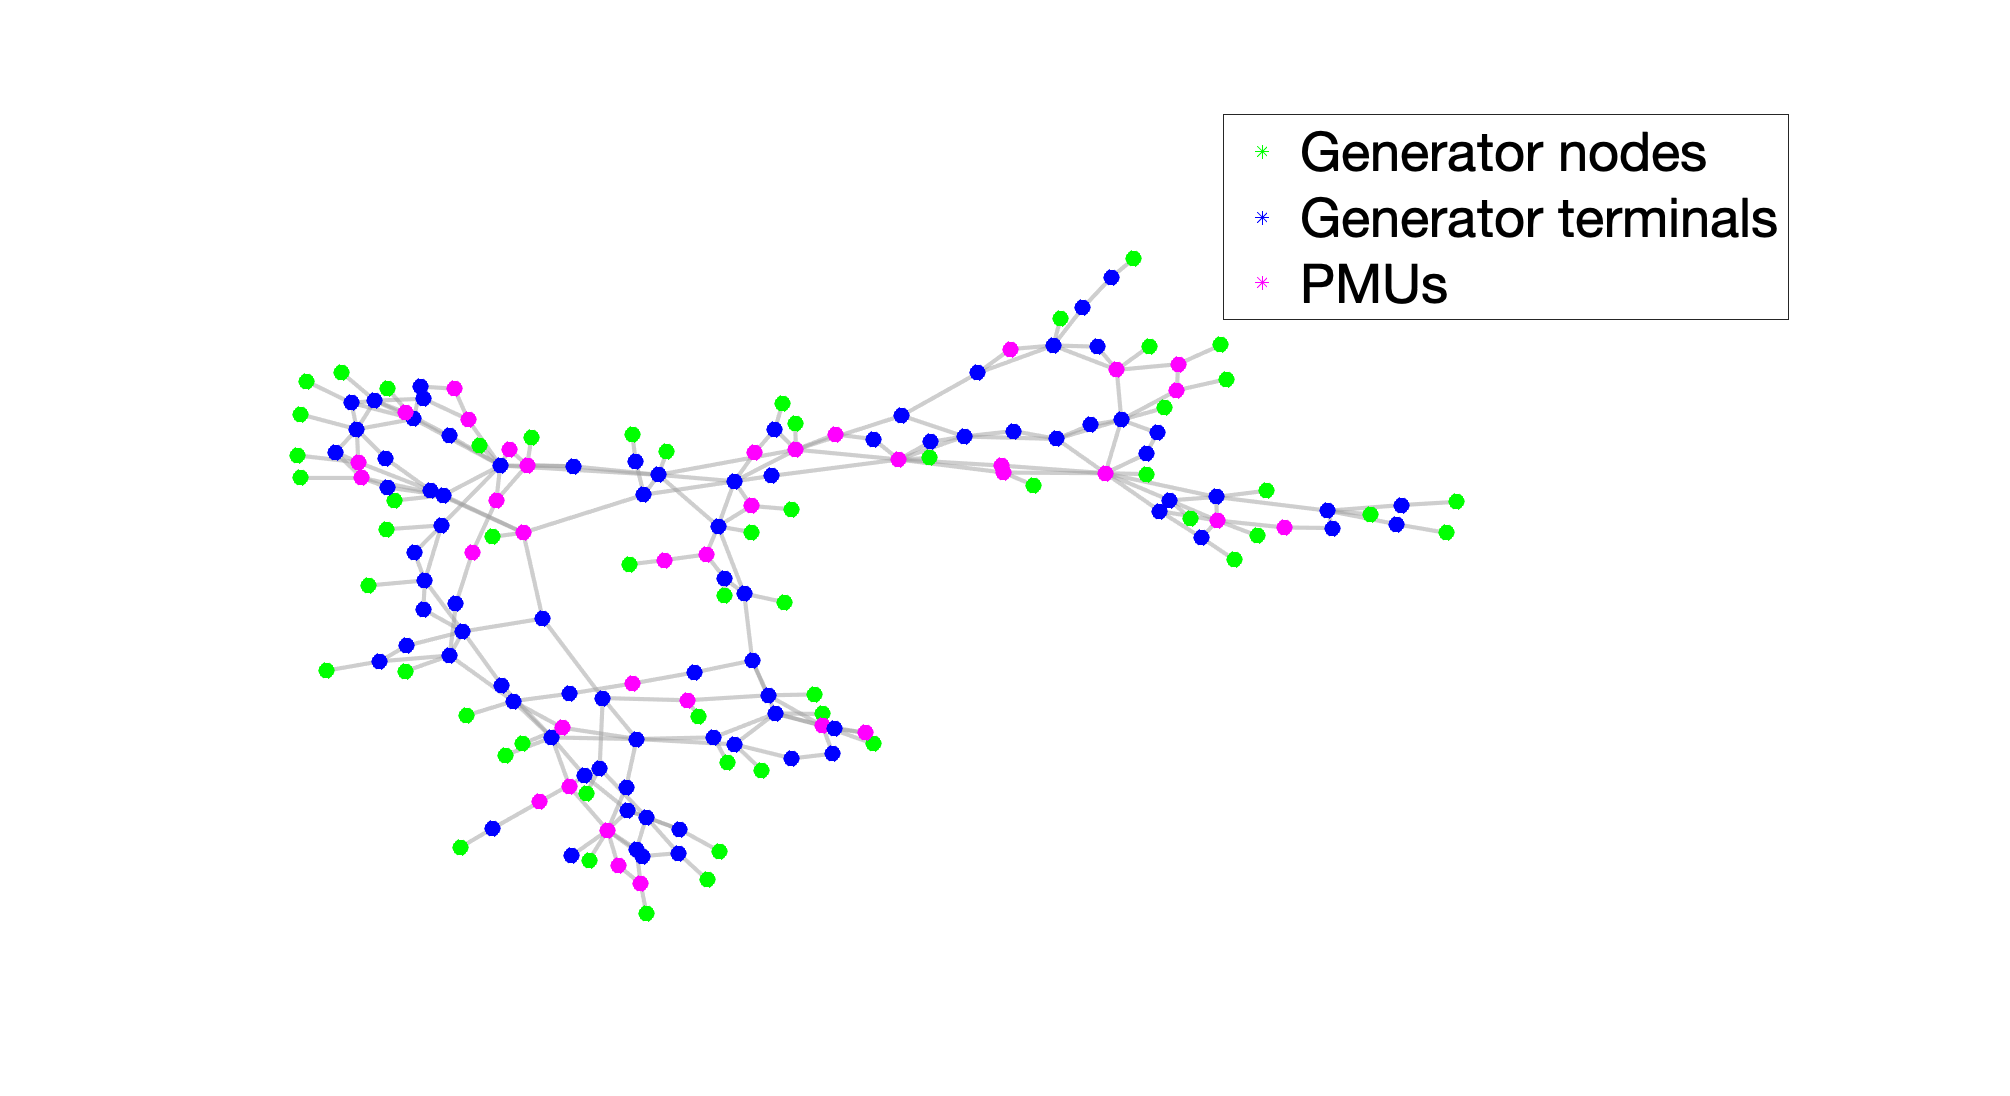
\includegraphics[width=\textheight]{graph-pg}
        \caption{IEEE 118 Power Grid's Dynamic Graph}%
        \label{fig:graph-pg}
      \end{figure}
    \end{column}%
  \end{columns}
\end{slide}

\begin{slide}{Functional Observer}
  \begin{columns}[c]
    \begin{column}{0.48\textwidth}
      \begin{itemize}
        \item \y{} are the measured outputs.
        \item \z{} are the states we wish to estimate.
        \item The observer has a reduced order dynamics system which is
              equivalent to the original one.
        \item Problem 1: how to find a \w{} that correctly estimates \z{}.
        \item Problem 2: how to find the observer's matrices \mN,\mJ,\mH and
              \mE.
      \end{itemize}
    \end{column}%
    \hfill%
    \begin{column}{0.48\textwidth}
      \begin{align}
        \begin{split}
          \dot{x}(t) & = Ax(t) + Bu(t) + Lf(t), \\
          \y         & = Cx(t),                 \\
          \z         & = Fx(t),
        \end{split} \\\nonumber\\
        \begin{split}
          \dw & = \mN\w + \mJ\y + \mH u(t), \\
          \hz & = \w + \mE\y.
        \end{split}
      \end{align}
    \end{column}%
  \end{columns}
\end{slide}

\begin{slide}{Observability}
  \begin{columns}[c]
    \begin{column}{0.48\textwidth}
      \begin{itemize}
        \item All desired states \z{} must be observable from the outputs \y.
        \item The observability of \((A,C,F)\) cannot be greater than that of
              \((A,C)\).
        \item There must be a path from every output \y{} to every output \z{}
              in the dynamics graph.
      \end{itemize}
    \end{column}%
    \hfill%
    \begin{column}{0.48\textwidth}
      \begin{equation}
        rank
        \begin{bmatrix}
          C \\ CA \\ F \\ FA
        \end{bmatrix}
        = rank
        \begin{bmatrix}
          C \\ CA \\ F
        \end{bmatrix}.
      \end{equation}
    \end{column}%
  \end{columns}
\end{slide}

\begin{slide}{Path Finder Algorithm}
  \begin{columns}[c]
    \begin{column}{0.48\textwidth}
      \begin{figure}[ht!]
        \centering \includegraphics[width=0.8\textwidth]{puma560}
        \caption{Puma 560}%
        \label{fig:puma}
      \end{figure}
    \end{column}%
    \hfill%
    \begin{column}{0.48\textwidth}
      \begin{figure}[ht!]
        \centering
        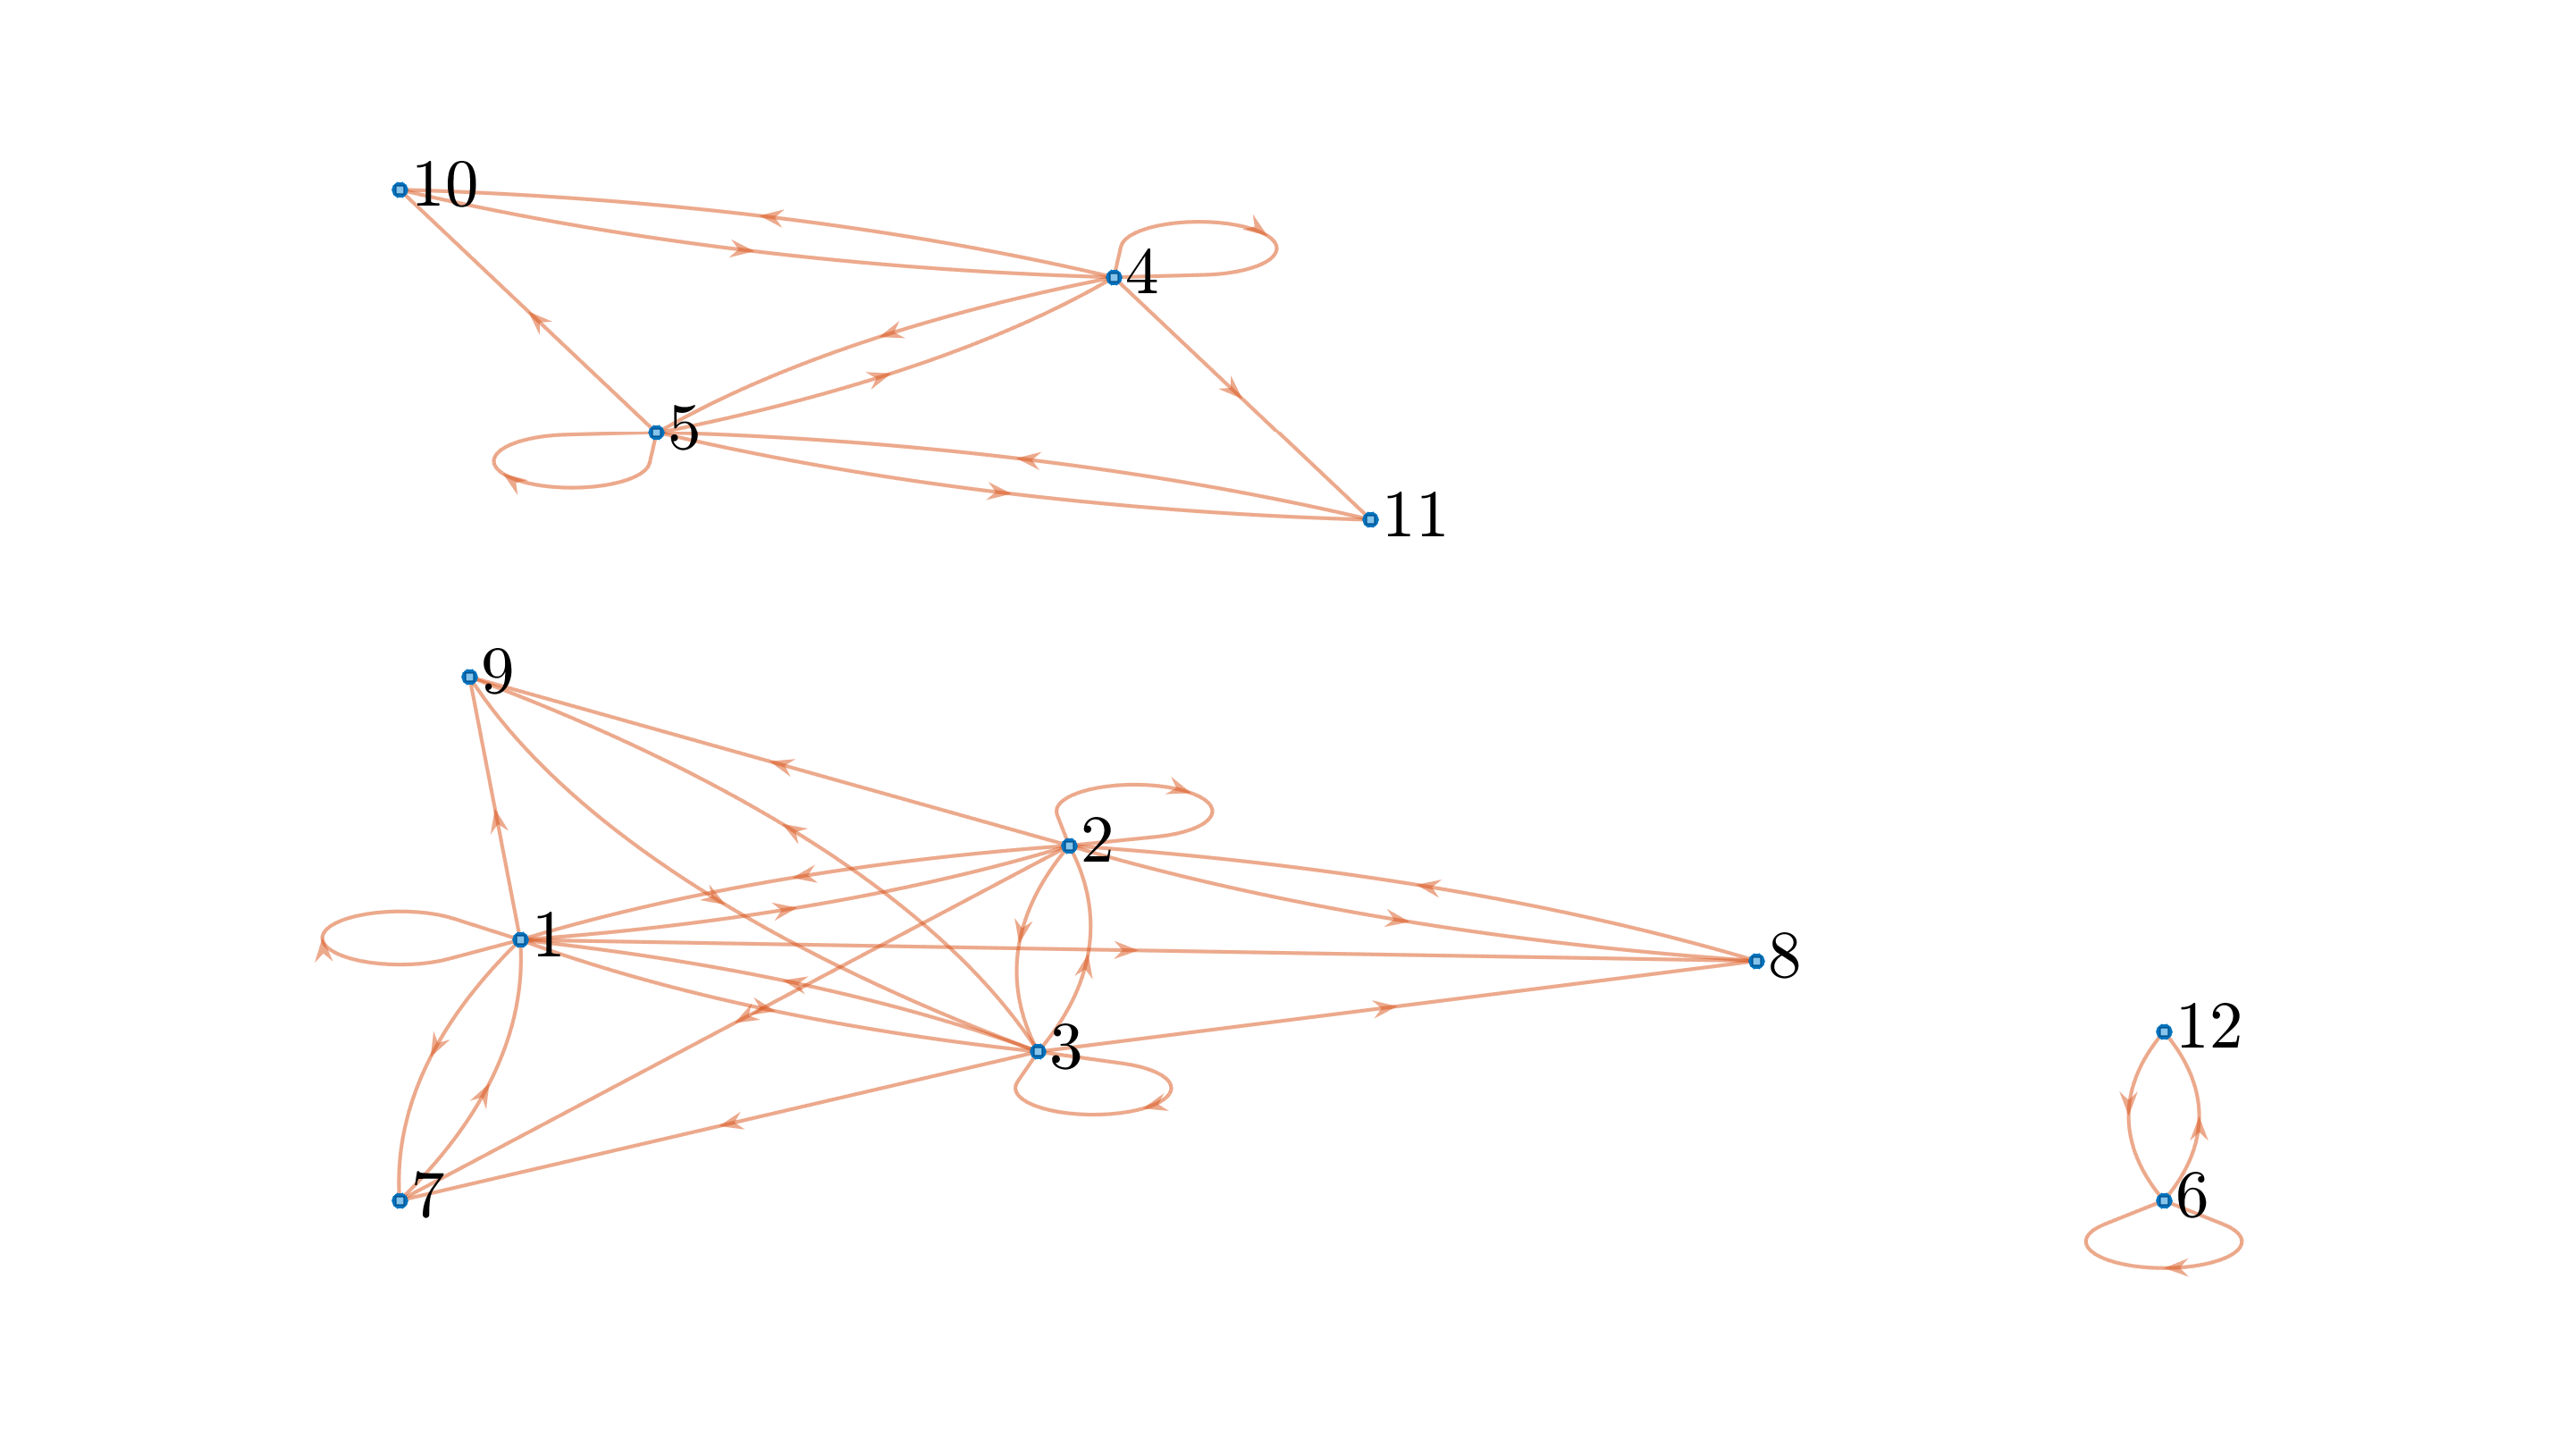
\includegraphics[width=\textwidth]{graph-puma}
        \caption{Puma 560 dynamic's graph representation.}%
        \label{fig:puma-graph}
      \end{figure}
    \end{column}%
  \end{columns}
\end{slide}
